%%%%%%%%%%%%%%%%%%%%%%%%%% AULA 01 %%%%%%%%%%%%%%%%%%%%%%%%%%

%%%%%%%%%%%%%%%%%%%%%%% FINALIDADE %%%%%%%%%%%%%%%%%%%%%%%%%%
%			Tratar das explicações básicas sobre o			%
%			TeX e LaTeX, apontando as principais			%
%			vantagens sobre os métodos comuns para a 		%
%			diagramação de documentos, além de demonstrar	%
%			comandos sobre formatação geral de documentos	%
%%%%%%%%%%%%%%%%%%%%%%% FIM FINALIDADE %%%%%%%%%%%%%%%%%%%%%%

%%%%%%%%%%% SLIDE 01 %%%%%%%%%%%%%%%%%%%%%%%%
\begin{frame}{O que é o \TeX?}
	\begin{itemize}
		\item \TeX~é um programa criado por Donald E.~Knuth, usado para desenvolvimento de documentos;
		\pause
		\item Formatador de documentos (como troff e groff -- programas hoje obsoletos);
	\end{itemize}
\end{frame}
%%%%%%%%%%% FIM SLIDE 01 %%%%%%%%%%%%%%%%%%%%

%%%%%%%%%%% SLIDE 02 %%%%%%%%%%%%%%%%%%%%%%%%
\begin{frame}{O que faz o \TeX?}
	\begin{itemize}
		\item Permite desenvolver documentos complexos, incluindo facilidades para:
		\pause
	\begin{itemize}
		\item Gerar sumário, index, lista de figuras, lista de tabelas e referências bibliográficas;
		\pause		
		\item Importar e tratar imagens de vários formatos  (escalando, rotacionando, convertendo, etc.);
		\pause
		\item Desenvolver gráficos diagramáticos;
		\pause
		\item Representar partituras musicais, partidas de xadrez, fórmulas químicas, dentre outros.
	\end{itemize}
\end{itemize}

	\pause
	\begin{Observacao}{O poder do \TeX}
		Reside em sua habilidade de tratar textos técnicos complicados e exibir fórmulas matemáticas.
	\end{Observacao}
\end{frame}
%%%%%%%%%%% FIM SLIDE 02 %%%%%%%%%%%%%%%%%%%%

%%%%%%%%%%% SLIDE 03 %%%%%%%%%%%%%%%%%%%%%%%%
\begin{frame}{Vantagens}
	\begin{itemize}
		\item Qualidade tipográfica superior (fontes e distribuição do texto na página);
		\pause
		\item Compatibilidade (Donald Knuth ``congelou'' o programa \TeX);
		\pause
		\item Estabilidade e ausência de falhas (uso prolongado do mesmo programa virtualmente eliminou todos os erros);
		\pause
		\item Padrão adotado pela \emph{American Mathematical Society} (AMS) para comunicação entre matemáticos;
		\pause
		\item Quantidade extremamente vasta de pacotes mantidos pela comunidade para facilitar qualquer tarefa.
	\end{itemize}
\end{frame}
%%%%%%%%%%% FIM SLIDE 03 %%%%%%%%%%%%%%%%%%%%%

%%%%%%%%%%% SLIDE 04 %%%%%%%%%%%%%%%%%%%%%%%%%
\begin{frame}{O que é \LaTeX?}
	\begin{itemize}
		\item \LaTeX\ é um conjunto padrão de macros para \TeX\ que permite um aumento da produtividade no uso do programa;
		\pause
		\item Mais macros podem ser incluidas por meio de pacotes (por exemplo: \Xy-pic, MusiX\TeX, CircuiTikz, etc.);
		\pause
		\item Programas externos, desenvolvidos por programadores e usuários de \TeX, extenderam as funcionalidades (por exemplo: BiB\TeX, makeindex, etc.).
	\end{itemize}
\end{frame}
%%%%%%%%%%% FIM SLIDE 04 %%%%%%%%%%%%%%%%%%%%%

%%%%%%%%%%% SLIDE 05 %%%%%%%%%%%%%%%%%%%%%%%%%
\begin{frame}{Abordagens para o projeto de documentos}
	\begin{itemize}
		\item Projeto visual $\times$ projeto lógico de documentos:
		\pause
		\begin{itemize}
			\item Projeto visual enfatiza o estético e envolve grande esforço de formatação;
			\pause
			\item Projeto lógico enfatiza a estrutura e economiza tempo pois a formatação é consequência da estrutura;
			\pause
			\item Projeto lógico provoca uma reflexão sobre o texto que tem consequências benéficas até sobre o conteúdo sendo desenvolvido;
		\end{itemize}
	\end{itemize}
\end{frame}
%%%%%%%%%%% FIM SLIDE 05 %%%%%%%%%%%%%%%%%%%%%

%%%%%%%%%%% SLIDE 06 %%%%%%%%%%%%%%%%%%%%%%%%%
\begin{frame}{Comparação entre processador de textos e \TeX}
	Fórmula obtida usando-se um processador de textos típico:
	\pause
	\begin{center}
		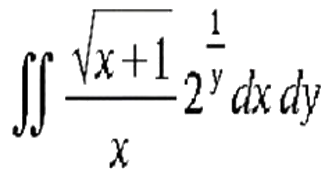
\includegraphics[width=0.5\textwidth, natwidth=326, natheight=175]{Imagens/integral.png}
	\end{center}

    \pause
	Fórmula obtida usando-se \TeX:
	\pause
	\[\int\!\!\!\int\frac{\sqrt{x+1}}{x}2^{\frac{1}{y}}\mathrm{d}x\,\mathrm{d}y\]
\end{frame}
%%%%%%%%%%% FIM SLIDE 06 %%%%%%%%%%%%%%%%%%%%%

%%%%%%%%%%% SLIDE 07 %%%%%%%%%%%%%%%%%%%%%%%%%
\begin{frame}{Projeto visual $\times$ lógico}
	\begin{description}
		\item [Projeto visual] baseado em menus e botões (o usuário ``desenha'' a fórmula/texto);
		\pause
		\item [Projeto lógico] baseado em comandos:
	\end{description}
	
	\pause
	
	\begin{Codigo}{Comandos}
		\string\[\LCmd{int}\string\!\string\!\string\!\LCmd{int}
		\LCmdArg{frac}{\LCmdArg{sqrt}{x+1}}\Larg{x}2\string^\{
		\LCmdArg{frac}{1}\Larg{y}\}\n
		\LCmdArg{mathrm}{d}x\string\,\LCmdArg{mathrm}{d}y\string\]
	\end{Codigo}

    \pause
	Produz:
    \begin{Resultado}{}
		\[\int\!\!\!\int\frac{\sqrt{x+1}}{x}2^{\frac{1}{y}}\mathrm{d}x\,\mathrm{d}y\]
    \end{Resultado}
\end{frame}
%%%%%%%%%%% FIM SLIDE 07 %%%%%%%%%%%%%%%%%%%%%

%%%%%%%%%%% SLIDE 08 %%%%%%%%%%%%%%%%%%%%%%%%%
\begin{frame}{Observações}
	\begin{itemize}
		\item \texttt{\string\[ } e \texttt{\string\]} -- entra e sai do modo matemático;
		\item \LCmd{int} -- integral;
		\item \texttt{\string\!} -- espaço negativo (para obter o espaçamento correto na integral dupla) -- poderia ter sido usado o comando \LCmd{iint};
		\item \LCmdArg{frac}{\ldots}\Larg{\ldots} -- fração;
		\item \LCmdArg{sqrt}{\ldots} -- raiz quadrada;
		\item \texttt{\string^} -- expoente;
		\item \texttt{\string\,} -- espaço pequeno;
		\item \LCmdArg{mathrm}{\ldots} -- fonte romano do modo matemático.
	\end{itemize}
\end{frame}
%%%%%%%%%%% FIM SLIDE 08 %%%%%%%%%%%%%%%%%%%%%

%%%%%%%%%%% SLIDE 09 %%%%%%%%%%%%%%%%%%%%%%%%%
\begin{frame}{Projeto lógico}
	\begin{itemize}
		\item No projeto lógico, o aspecto estético depende do contexto/estrutura (por exemplo, se a fórmula está dentro de um parágrafo ou destacada do parágrafo). 
		Exemplo:
		\begin{itemize}
			\item O somatório $\sum_{i = 0}^\infty a_i/2$ resulta em \dots
			\pause	
			\item O somatório $$\sum_{i = 0}^\infty \frac{a_i}{2}$$ resulta em \dots
		\end{itemize}
	\end{itemize}
\end{frame}
%%%%%%%%%%% FIM SLIDE 09 %%%%%%%%%%%%%%%%%%%%%